\chapter{Tietoturva}\label{tietoturva}

Tietoturvalla tarkoitetaan tietokonejärjestelmien ja verkkojen suojelemista elektronisten resurssien varkauksilta, ohjelmistojen ja laitteiden vahingoilta sekä tahallaan aiheutetuilta häiriöiltä palvelujen toimintakyvyssä. Suojautumaan pyritään myös palvelujen väärinkäytöksiltä. Tietoturvan merkitys on kasvanut nopeasti digitalisaation myötä.~\cite{andress2014basics}

\section{CIA-malli}\label{cia_malli}

Tärkeimpiä konsepteja tietoturvasta puhuttaessa on luottamuksellisuus, eheys sekä saatavuus. Tämän johdosta yksi tärkeimmistä malleista kuvata tietoturvan osa-alueita on CIA-malli (Confidentality, Integrity, Availability). Malli antaa viitekehyksen keskustellessa siitä, millainen jokin tietoturvauhka on. Mallin mukaisesti jokin tietoturvauhka kohdistuu aina yhteen tai useampaan CIA-mallin osa-alueista.

ISO/IEC 27000:2018(E) -standardi~\cite{ISO27000} määrittelee CIA-mallin kohdat seuraavasti:

\begin{itemize}
    \item \textbf{Luottamuksellisuus}: ``Property that information is not made available or disclosed to unauthorized individuals, entities, or processes''
    \item \textbf{Eheys}: ``Property of accuracy and completeness''
    \item \textbf{Saatavuus}: ``Property of being accessible and usable on demand by an authorized entity''
\end{itemize}

Luottamuksellisuudella tarkoitetaan siis sitä, että tietoa voivat nähdä vain ne, joilla on siihen oikeus. Eheys on sitä, että tiedon oikeuden ja täydellisyyden varmistamista siltä, että tietoa muokattaisiin luvattomasti. Saatavuudella puolestaan tarkoitetaan sitä, että tieto on saavutettavissa siihen oikeutettujen tahojen toimesta.~\cite{stamp2011information}

\section{Haavoittuvuudet ja kyberhyökkäykset}\label{haavoittuvuudet_ja_kyberhyokkaykset}
Tietoturva-aukolla eli haavoittuvuudella tarkoitetaan heikkoutta tietokonejärjestelmässä, jonka avulla hyökkääjän on mahdollista päästä tekemään järjestelmässä jotakin mitä hänen ei pitäisi. Kyberhyökkäys tarkoittaa varsinaista toimenpidettä, jossa hyökkääjä käyttää haavoittuvuutta päästäkseen järjestelmään.~\cite{andress2014basics}

Esittelen seuraavaksi yleisimpiä kyberhyökkäyksiä, mitä haavoittuvuutta ne hyödyntävät ja mitä CIA-mallin kohtaa ne vaarantavat. Merkitsen jokaisen esittelemäni hyökkäyksen tunnisteella ja numeroinnilla Hx, jotta niihin on helpompi palata myöhemmissä luvuissa.

\subsection{H1: Palvelunestohyökkäys}\customlabel{dos}{H1}
Palvelunestohyökkäyksen (eng. \textit{Denial of Service, DoS}) tarkoitus on saada jokin verkossa oleva resurssi pois käytöstä häiritsemällä tätä internetin välityksellä. Tyypillisesti tämä saavutetaan häiritsemällä kohdetta lukuisilla palvelupyynnöillä, joiden tarkoitus on saada resurssi ylikuormitettua, jonka jälkeen tavalliset resurssin käyttäjät eivät enää pääse tähän käsiksi. Palvelunestohyökkäys estää palvelun saatavuuden, joten se hyökkää CIA-mallin A-kohtaan.

Palvelintietokoneella on lukuisia rajallisia resursseja kuten kaista, levytila tai suoritinaika. Hyökkääjä voi esimerkiksi lähettää toistuvasti palvelupyyntöjä ladatakseen suuren tiedoston palvelimelta ja näin ollen tukkia kaistan tai hyökkääjä voi lähettää toistuvia palvelupyyntöjä johonkin resurssiin, jonka tietää olevan raskas suorittimelle ja näin ollen ylikuormittaa suorittimen.

Todellisuudessa harvalla hyökkääjällä on käytössään sellaisia resursseja, joilla olisi mahdollista tukkia jonkin kaupallisen toimijan palvelinresurssit. Tämän vuoksi nykyään yleisempi tapa toteuttaa palvelunestohyökkäys on tehdä se hajautetusti (DDoS, Distibuted Denial of Service). Hajautetussa palvelunestohyökkäyksessä hyökkääjällä on käytössään useista internetiin yhdistetyistä tietokoneista muodostuva bottiverkko.~\cite{nist_ddos}

Kuvassa~\ref{github_ddos} toistaiseksi toiseksi suurimman palvelunestohyökkäyksen piikki kaistankäytössä hyökkäyksen aikana. Hyökkäys on vuodelta 2018 ja se kohdistui GitHubiin. Poikkeuksellisesti hyökkäyksessä ei käytetty bottiverkkoa vaan hyökkääjä vahvisti omia häirintäpyyntöjään useilla tuhansilla väärinkonfiguroiduilla Memcached-palvelimilla.~\cite{github_ddos}

\begin{figure}
\centering 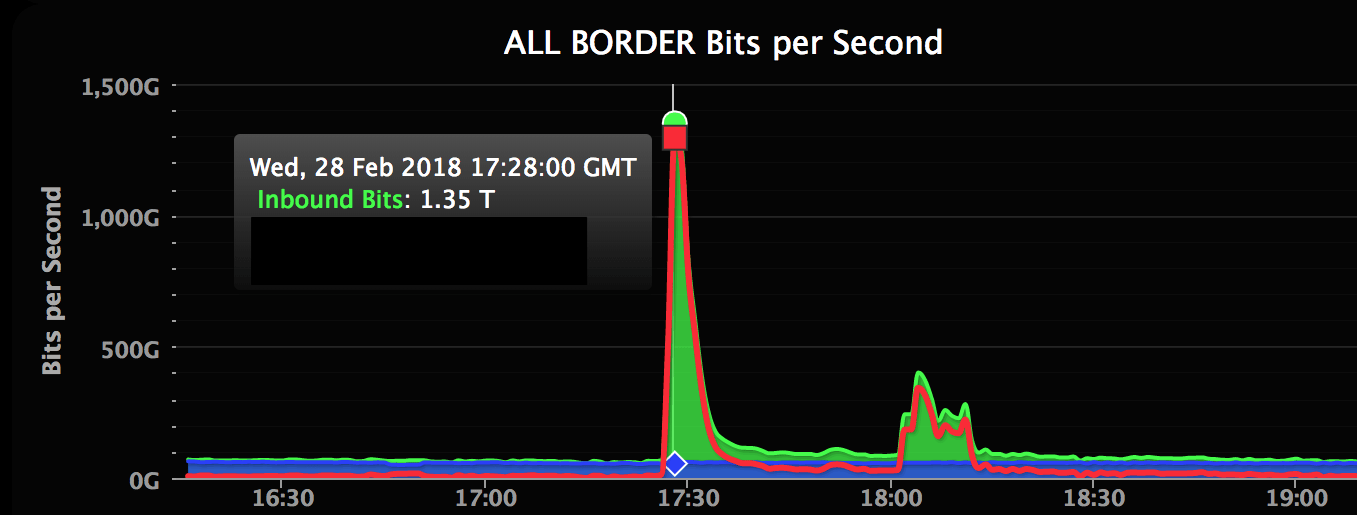
\includegraphics[width=1\textwidth]{kuvat/github_ddos.png}
\caption{Github DDoS 2018~\cite{github_ddos}}
\label{github_ddos} 
\end{figure}

\subsection{H2: Takaovet}\customlabel{backdoors}{H2}
Takaovi (eng. \textit{Backdoor}) on keino ohittaa järjestelmän tyypilliset autentikointimenetelmät. Tyypillisesti takaovi on tietokoneohjelma joka antaa hyökkääjälle hallinnan kohdejärjestelmästään. Esimerkiksi Linux-järjestelmässä takaovella yritetään saada tilanne aikaan, jossa hyökkääjä voi kirjautua sisään kohdejärjestelmälle \textit{root}-oikeuksilla käymättä kuitenkaan läpi normaalia autentikaatioprosessia. Takaovi on ylimääräinen ohjelma, jonka ei kuuluisi olla kohdejärjestelmässä, joten lähtökohtaisesti takaovi vaarantaa CIA-mallin I-osan. Mikäli takaovi mahdollistaa hyökkääjälle \textit{root}-käyttäjän oikeudet, hyökkääjällä on täysi hallinta kohdejärjestelmästä. Edellä mainitun tilanteen voi katsoa vaarantavan kaikki CIA-mallin osa-alueet.

Takaovi asennetaan kohdetietokoneelle esimerkiksi nk.\ troijalaisen mukana. Troijalainen on viattomaksi naamioitu haittaohjelma, esimerkiksi peli, jonka mukana on kuitenkin ohjelmakoodia, joka ei kuulu peliin kuten esimerkiksi takaovi.

Takaovia asennetaan myös jo muilla keinoin onnistuneen hyökkäyksen päätteeksi taatakseen hyökkääjällä pääsyn kohdejärjestelmään tulevaisuudessa.~\cite{tipton2007information}

\subsection{H3: Verkon kuuntelu}\customlabel{verkon_kuuntelu}{H3}
Verkon kuuntelu (eng. \textit{Network Eavesdropping}) on keino salakuunnella jotakin tahoa analysoimalla verkkoliikennettä. Useimmiten liikenne on salattu, joten ensin on onnistuttava murtautumaan salauksen läpi. Liikenne voi myös kulkea kaapeleita pitkin, joihin pääsy on fyysisesti estetty ja itse verkkoliikenne on salaamatonta. Verkon kuuntelulla lähtökohtaisesti hyökätään CIA-mallin C-kohtaan, sillä hyökkääjä näkee tietoja, jotka eivät ole hänen katseltavakseen tarkoitettu. Verkon kuuntelun tuloksena voidaan saada käsiin tietoja, joilla onnistutaan tekemään jokin muu kyberhyökkäys.

Langattomien verkkojen aikana verkon kuuntelu ei vaadi enää fyysistä pääsyä kaapeleihin, joten tarpeeksi suurella vastaanottimella hyökkääjä voi toteuttaa hyökkäyksen hyvinkin kaukaa. Tätä ongelmaa on korjattu vahvoilla salauksilla langattomassa verkkoliikenteessä. Varsinkin WLAN:n alkuaikoina salaukset olivat heikkoja tai niitä ei ollut lainkaan ja tämä oli suuri ongelma.~\cite{andress2014basics}

\subsection{H4: Eskalaatiohyökkäys}\customlabel{privilege_escalation}{H4}
Eskalaatiohyökkäys (eng. \textit{Privilege escalation}) on keino saada ylimääräisiä käyttäjäoikeuksia ja näin päästä käsiksi resursseihin, joihin kyseinen käyttäjä ei normaalisti olisi oikeutettu. Tyypillisesti tämä toteutetaan hyödyntämällä bugia, suunnitteluvirhettä tai konfigurointivirhettä käyttöjärjestelmässä tai sovelluksessa.

Käyttöoikeuksien eskalaatio voi tapahtua joko vertikaalisesti tai horisontaalisesti. Vertikaalisessa eskalaatiohyökkäyksessä pyritään saamaan korkeampia käyttöoikeuksia kun taas horisontaalisessa eskalaatiohyökkäyksessä pyritään saaamaan jonkun toisen saman tason käyttäjän oikeuksia. Linux-järjestelmissä vertikaalisessa eskalaatiohyökkäyksessä yritetään tyypillisesti saada \textit{root}-käyttäjän oikeudet.~\cite{ciampa2012security+}

\begin{figure}
\centering 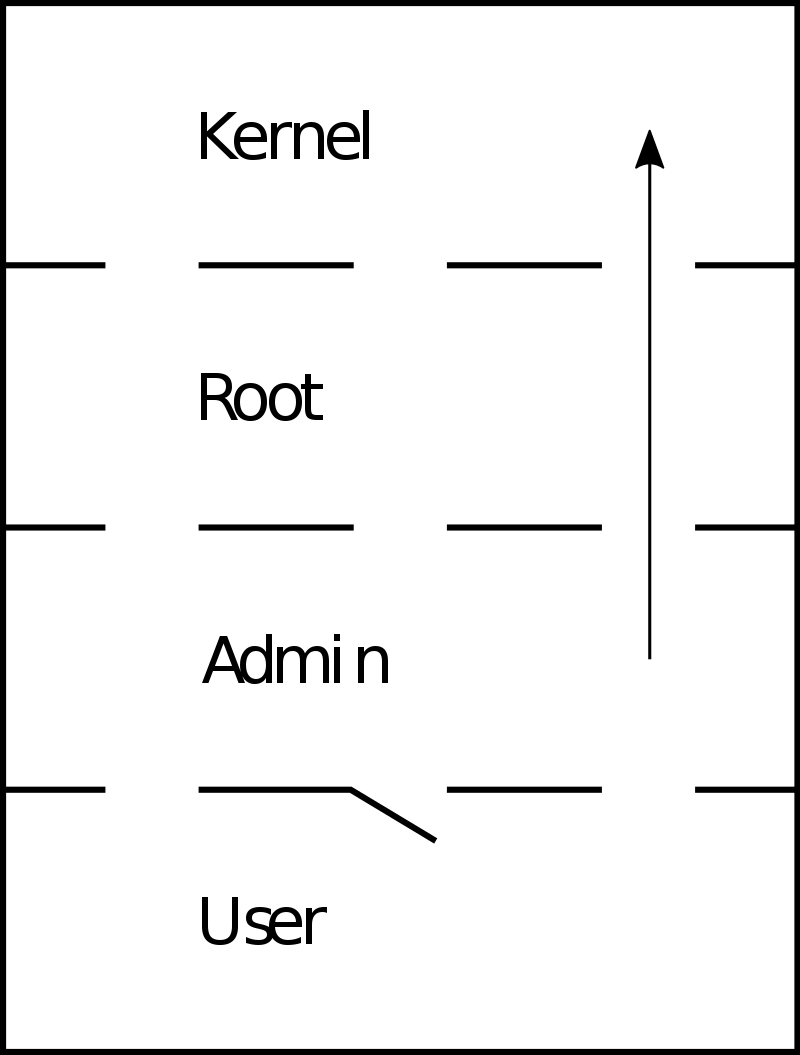
\includegraphics[width=0.25\textwidth]{kuvat/privilege_escalation.png}
\caption{Diagrammi eskalaatiohyökkäyksestä~\cite{wikipedia:privilege_escalation}}
\label{privilege_escalation_diagram} 
\end{figure}

\subsection{H5: Injektiohyökkäys}\customlabel{injection}{H5}
Injektiohyökkyksessä (eng. \textit{Code Injection}) hyökkääjä onnistuu haavoittuvuuden avulla suorittamaan kohdejärjestelmässä koodia, jota hänen ei olisi tarkoitus pystyä suorittamaan. Haavoittuvuus johtuu ohjelmointivirheestä ja tyypillisesti tilanteissa, jossa palvelin prosessoi käyttäjän syötettä ja tätä syötettä ei sarjoiteta oikein. Injektiohyökkäys voi pahimmillaan ja varsinkin hyökkäyksen \ref{privilege_escalation} kanssa johtaa kohteen täyden kontrollin päätymiseen hyökkääjälle, joten injektiohyökkäys vaarantaa CIA-mallin jokaisen kohdan. Erilaisia injektiohyökkäyksiä ovat mm. SQL-injektio, web-sovelluksen ohjelmointikielen (esim. PHP) injektio ja sivustojen välinen skriptaus (eng. \textit{Cross-site scripting}).

Verkkosovellukset ovat usein injektiohyökkäyksen kohteena. Haavoittuvuus on useimmiten web-sovelluksessa, mutta saattaa olla myös palvelinsovelluksessa. Tyypillisessä haavoittuvuudessa web-sovellus prosessoi verkkosivuston käyttäjän syötettä ilman minkäänlaista validointia tai hyvin vähäisellä sellaisella.~\cite{mcdonald2020web}

\subsection{H6: Väsytyshyökkäys}\customlabel{bruteforce}{H6}
Väsytyshyökkäyksessä (eng. \textit{Brute-force attack}) hyökkääjä käy systemaattisesti läpi kaikki mahdolliset vaihtoehdot salasanan tai salausavaimen arvaamiseksi. Salasana, jota yritetään arvata, voi olla esimerkiksi Linuxin käyttöjärjestelmän käyttäjän salasana tai salauksen purkuun tarvittava salasana. Väsytyshyökkäyksellä pyritään arvaamaan jokin tieto, joka ei ole tarkoitettu hyökkääjän nähtäväksi, joten väsytyshyökkäys vaarantaa CIA-mallin kohdan C.

Jotta väsytyshyökkäys voitaisiin toteuttaa kohteen ei tulisi asettaa rajoituksia sille kuinka monta kertaa salasanaa voidaan kokeilla ja jotta hyökkäys voitaisiin toteuttaa kohtuullisessa ajassa, eri salasanojen kokeilu pitäisi onnistua tekemään nopeasti. Käytännössä mikä tahansa salasana on arvattavissa mikäli salasanan kokeilukertoja ei ole rajoitettu. Tämä voi tosin viedä epäkäytännöllisen pitkän ajan kuten esimerkiksi tuhansia vuosia.

Väsytyshyökkäystä voidaan tehostaa monin tekniikoin kuten esimerkiksi sanalistoilla. Ihmisten valitsemat salasanat ovat yleensä luonnollisten kielien sanoja tai niiden yhdistelmiä tai muunnelmia. Väsytyshyökkäyksessä voidaan kokeilla ensin nämä ja jos tämä ei onnistu niin jatkaa satunnaisten merkkijonojen kokeiluun.~\cite{beaver2015hacking}

\subsection{H7: Laitteen varkaus}\customlabel{theft}{H7}
Tietoturvan kontekstissa laitteen varkaudella pyritään saamaan haltuun tietoa jota laitteilla säilytetään. Tällainen laite voi olla esimerkiksi kannettava tietokone, muistitikku tai palvelinsalin hävitettäväksi menossa oleva kovalevy. Tieto johon hyökkääjä haluaa päästä käsiksi voi olla jo suoraan varastettavalla laittella tai varastettava laite voi sisältää vain esimerkiksi salasanan tai salausavaimen, jota voi käyttää murtautumaan jollekin muulle resurssille. Tyypillisesti laitteen varkaus vaarantaa CIA-mallin kohdan C-kohdan, sillä hyökkääjä pyrkii pääsemään käsiksi tietoon johon hänellä ei ole oikeuksia. Toisaalta, mikäli laite varastetaan sen toivossa, että se sisältäisi esimerkiksi jonkin palvelimen käyttäjän salasanan niin laitteen varkaus voi vaarantaa CIA-mallin kaikki kohdat.~\cite{beaver2015hacking}
